%%%%%%%%%%%%%%%%%%%%%%%%%%%%%%%%%%%%%%%%%%%%%%%%%%%%%%%%%%%%%%%%%%%%%%%%%%%%
%
%		Relazione del progetto di Sistemi Distribuiti: Paradigmi e Modelli
%
%				    Nicola Corti - 2013
%
%%%%%%%%%%%%%%%%%%%%%%%%%%%%%%%%%%%%%%%%%%%%%%%%%%%%%%%%%%%%%%%%%%%%%%%%%%5%
\documentclass[a4paper,10pt]{article} 
\usepackage{graphicx}
\usepackage{vmargin}
\usepackage[italian]{babel} 
\usepackage[utf8x]{inputenc}
\usepackage{listings}
\usepackage{url}
\usepackage{pdflscape}
\usepackage{hyperref}
\usepackage[usenames,dvipsnames,svgnames,table]{xcolor}




\setpapersize{A4}
\setmarginsrb{15mm}{10mm}{15mm}{10mm}%
             {0mm}{10mm}{0mm}{10mm}

\lstset{
basicstyle=\small\ttfamily,
keywordstyle=\color{MidnightBlue}\bfseries,
identifierstyle=\color{Black},
commentstyle=\color{Green}\itshape,
stringstyle=\color{Red}\ttfamily,
showstringspaces=false,
%numbers=left, numberstyle=\tiny,
%stepnumber=1, numbersep=10pt,
tabsize=4,
framexleftmargin=5mm, rulesepcolor=\color{Gray},
frame=tb,
backgroundcolor=\color{LightGray},
language={Java},
%mathescape=true,
%fontadjust=true,
%breaklines=true,breakatwhitespace=true,breakautoindent
}


\title{Histogram Thresholding - Implementazione per architetture multicore tramite il framework Skandium}
\author{Nicola Corti - 454413 \\Corso di Laurea Magistrale in Informatica - Universit\`a di pisa}
\date{20 Settembre 2013}

\renewcommand\lstlistingname{Codice}
\renewcommand\figurename{Immagine}
 
\begin{document}
\maketitle
 
\begin{abstract}
Questa relazione ha lo scopo di illustrare i dettagli relativi alla progettazione, alla realizzazione e all'uso di \textsf{Histogram}: un software per il calcolo dell'Histogram Thresholding di un'immagine implementato per piattaforme multicore grazie all'utilizzo del framework Java Skandium.
\end{abstract}

\tableofcontents

\section*{Introduzione}

La realizzazione del software ha avuto come fare iniziale quella di design (sezione \ref{sec:design}) in cui sono state valutate le varie alternative per  la soluzione del problema e sono state prese le scelte che hanno portato alla fase di implementazione (sezione \ref{sec:implementation}): il software \`e stato realizzato in Java utilizzando il framework Skandium per supportare l'esecuzione su piattaforme parallele.

Successivamente si \`e provveduto a valutare le performance (sezione \ref{sec:performance}) del software su piattaforme con configurazioni differenti al fine di valutare la bont\`a del modello descritto nella fase di design.

La fase di sviluppo del software \`e terminata con la realizzazione di un archivio contenente i sorgenti, la documentazione annessa e la guida utente (sezione \ref{sec:userguide}) rivolta ad ogni utente che volesse utilizzare il software.

\section{Design}
\label{sec:design}

La fase di design ha avuto come punto di partenza l'individuazione di un algoritmo sequenziale che effettuasse il calcolo dell'histogram thresholding su una singola matrice, in modo da poterlo utilizzare come punto di partenza per definire il modello parallelo.

\subsection{Gli algoritmi sequenziali}

Sono stati individuati due differenti algoritmi sequenziali: il primo, pi\`u inefficiente, ha un costo quadratico rispetto al numero degli elementi di una matrice, il secondo invece \`e pi\`u efficiente ed ha un costo lineare nel numero degli elementi della matrice.

I due algoritmi verranno presentati in dettaglio nei paragrafi seguenti:

\subsubsection{Algoritmo Quadratico}

L'algoritmo quadratico ricalca la definizione del problema: per ogni elemento della matrice considerata si vanno a contare quanti sono gli elementi della stessa matrice che sono maggiori (minori). Si va a settare a 0 o ad 1 il corrispettivo bit della matrice risultante in base al fatto che il conteggio sia superiore o inferiore alla percentuale di soglia.

L'algoritmo \`e presentato sinteticamente nel seguente pseudo codice:

\begin{lstlisting}[backgroundcolor=\color{White}, caption={Pseudo codice dell'algoritmo quadratico}]
soglia = threshold * (mat.righe * mat.colonne)

for(i = 0; i < mat.righe; i++){
	for(j = 0; j < mat.colonne; j++){
	
		// Considero un generico elemento
		conta = 0;
		
		// Conteggio i valori maggiori
		for(k = 0; k < mat.righe; k++){
			for(l = 0; l < mat.colonne; l++){
				if (mat[i][j] > mat[k][l]) conta++;
			}
		}
		
		// Aggiorno di conseguenza la matrice risultante
		if (conta > soglia)
			res[i][j] = 0;
		else
			res[i][j] = 1;
	}
}
\end{lstlisting}

\paragraph{Osservazioni}

Si noti come questo algoritmo abbia bisogno di utilizzare una matrice risultate e non sia possibile aggiornare direttamente i valori della matrice della partenza; ci\`o porterebbe infatti ad un'inconsistenza e dunque all'impossibilit\`a di procedere al conteggio sequenziale di ogni singolo elemento.

Il seguente algoritmo ha un costo pari ad $O((n \times m)^2)$ per una matrice di dimensione $n \times m$

\subsubsection{Algoritmo Lineare}

L'algoritmo lineare procede invece in tre fasi:
\begin{enumerate}
\item Viene inizialmente costruito un istogramma dell'immagine: si utilizza un array dove si calcolano le frequenze di ogni singolo valore della matrice (vedi immagine \ref{img:histogram}),
\item Partendo dall'istogramma viene calcolato il valore numerico della soglia,
\item Nella seconda fase si scandisce linearmente la matrice di partenza e si impostano i bit a 0 o ad 1 in base al fatto che il singolo elemento sia superiore o minore rispetto al valore di soglia precedentemente calcolato.
\end{enumerate}

\begin{figure}[ht]
\centering
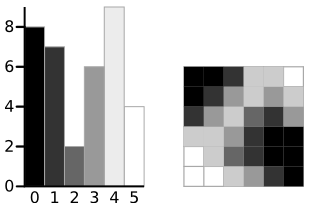
\includegraphics[height=4cm]{histo.png}
\caption{Esempio del calcolo dell'istogramma su una matrice $6 \times 6$ con valori da 0 a 5 (rappresentati con gradazioni di grigio)}
\label{img:histogram}
\end{figure}

L'algoritmo \`e presentato sinteticamente nel seguente pseudo codice:

\begin{lstlisting}[backgroundcolor=\color{White}, caption={Pseudo codice dell'algoritmo lineare}]
// Calcolo dell'istogramma
for(i = 0; i < mat.righe; i++){
	for(j = 0; j < mat.colonne; j++){
		isto[mat[i][j]]++;
	}
}

// Calcolo del valore di soglia
soglia = threshold * (mat.righe * mat.colonne)
risultato = 0; conta = 0;

while (risultato < isto.max AND conta < soglia){
	conta = conta + isto[risultato];
	risultato++;		
}

// Aggiornamento della matrice
for(i = 0; i < mat.righe; i++){
	for(j = 0; j < mat.colonne; j++){
		if (mat[i][j] < risultato)
			mat[i][j] = 0;
		else
			mat[i][j] = 1;
	}
}
\end{lstlisting}

\paragraph{Osservazioni}

Si noti come questo algoritmo, a differenza del precedente, effettua semplicemente due visite lineari di tutta la matrice; inoltre non necessita di una matrice di appoggio, ma pu\`o aggiornare direttamente la matrice di partenza, una volta calcolato il valore numerico di soglia.

Il seguente algoritmo ha un costo invece pari ad $O(n \times m)$ per una matrice di dimensione $n \times m$

\subsection{I modelli paralleli}

Partendo dai due algoritmi sequenziali sono stati proposti differenti modelli che verranno presentati nelle sezioni seguenti.

\subsubsection{Modello per l'algoritmo quadratico}

L'algoritmo sequenziale quadratico pu\`o essere parallelizzato tramite l'utilizzo di una \textsf{Map}: si divide la matrice di partenza per righe (colonne) ed ogni porzione di matrice viene assegnata ad un worker differente (immagine \ref{img:map}).

Ogni worker provveder\`a a calcolare la propria porzione di matrice, utilizzando la matrice di partenza per effettuare i conteggi.

Il calcolo termina quando tutti gli worker hanno terminato di calcolare la propria porzione.

\begin{figure}[ht]
\centering
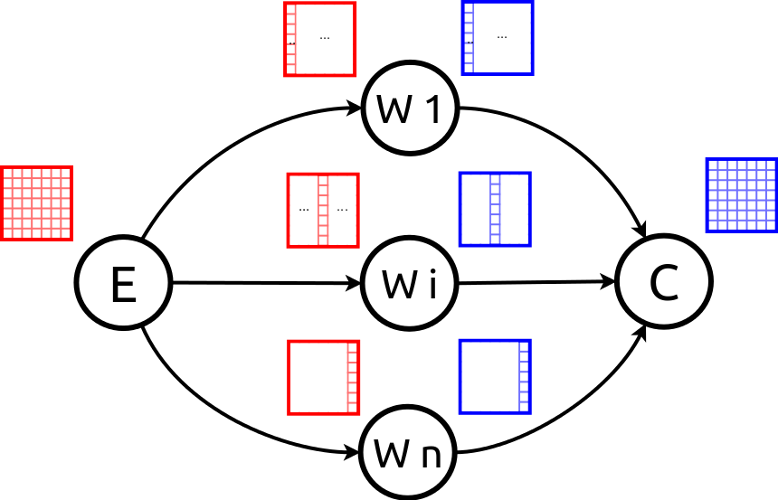
\includegraphics[height=5cm]{map.png}
\caption{Rappresentazione grafica del modello \textsf{Map}, le matrici rosse rappresentano le matrici con i valori di partenza, le matrici blu rappresentano matrici di 0 o 1.}
\label{img:map}
\end{figure}

\subsubsection{Modello per l'algoritmo lineare}

Per l'algoritmo lineare sono stati individuati due modelli differenti:

\paragraph{Modello \textsf{Pipeline}}
Il primo modello individuato consiste nel realizzare un \textsf{Pipeline} a due stadi (immagine \ref{img:pipeline}):

\begin{itemize}
\item Il primo stadio \`e una \textsf{Map-Reduce} che si occupa di calcolare l'istogramma in modo parallelo nella fase di {Map}, di ricomporlo nella fase di {Reduce} e successivamente di calcolare il valore di soglia,
\item Il secondo stadio \`e una \textsf{Map} che si occupa di aggiornare in modo parallelo la matrice in base al valore di soglia calcolato nello stadio precedente.
\end{itemize}

L'utilizzo di un pipeline permette di gestire in modo ottimale uno stream di matrici in entrata.

\begin{figure}[ht]
\centering
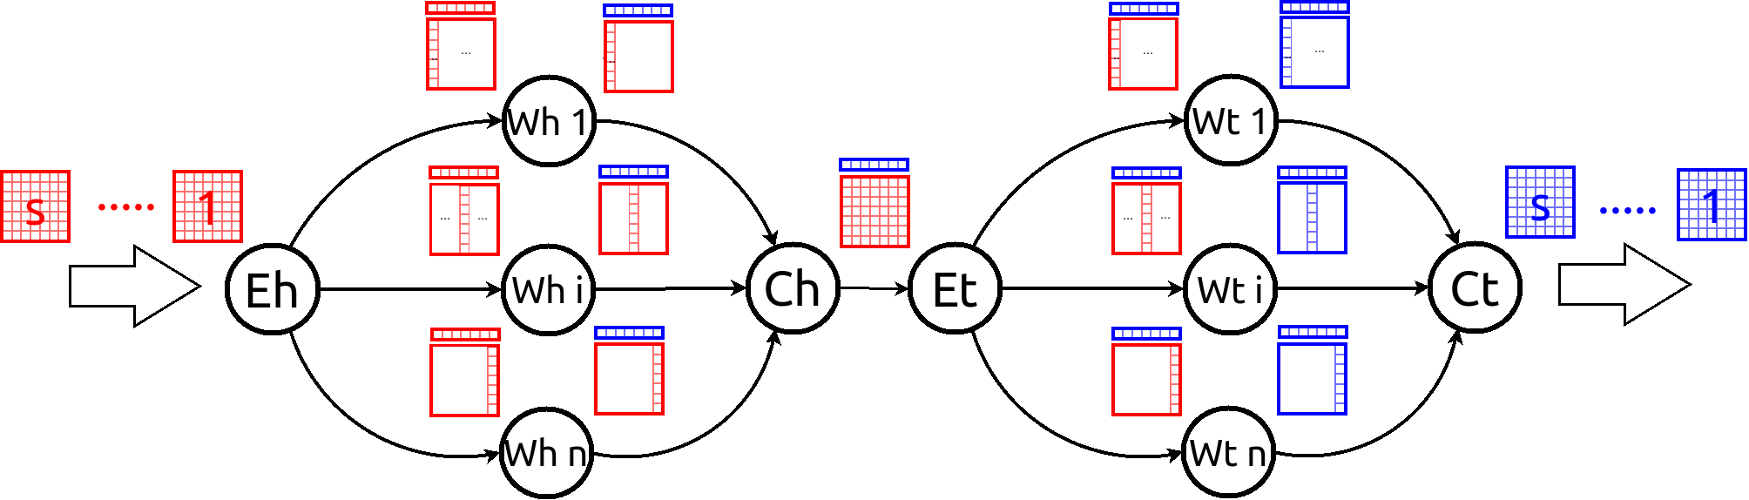
\includegraphics[height=4cm]{pipeline.png}
\caption{Rappresentazione grafica del modello \textsf{Pipeline}, le matrici rosse rappresentano le matrici con i valori di partenza, le matrici blu rappresentano matrici di 0 o 1. I piccoli vettori rappresentano gli istogrammi delle matrici, rossi se non sono stati calcolati, blu altrimenti}
\label{img:pipeline}
\end{figure}


\paragraph{Modello \textsf{Farm}}
Il secondo modello considera una grana del calcolo pi\`u grossolana, realizzando un \textsf{Farm}: ogni worker si occupa di effettuare tutte le 3 fasi dell'algoritmo lineare, ognuno su una matrice distinta (immagine \ref{img:farm}).

Anche con il modello \textsf{Farm} si riesce a gestire in modo ottimale uno stream di matrici in entrata.

\begin{figure}[ht]
\centering
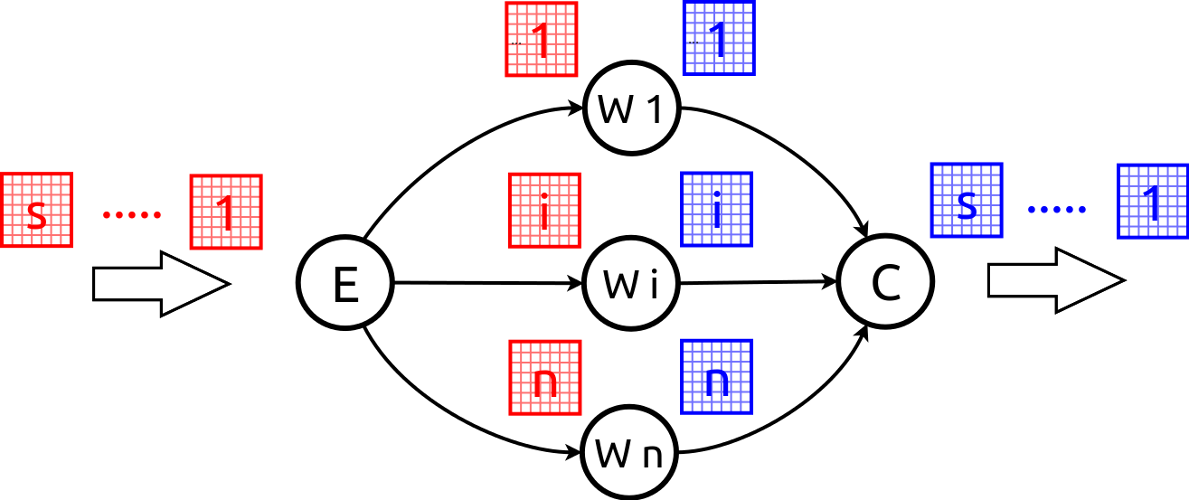
\includegraphics[height=5cm]{farm.png}
\caption{Rappresentazione grafica del modello \textsf{Farm}, le matrici rosse rappresentano le matrici con i valori di partenza, le matrici blu rappresentano matrici di 0 o 1.}
\label{img:farm}
\end{figure}


\section{Implementation}
\label{sec:implementation}

Il software \`e stato realizzato in Java, utilizzando il framework parallelo Skandium\footnote{https://github.com/mleyton/Skandium}, che offre un ambiente per la realizzazione di applicazioni parallele utilizzando gli skeleton pi\`u comuni.

Nei paragrafi seguenti sono descritti tutti i dettagli implementativi e le scelte prese al fine di rendere pi\`u facile la comprensione del codice.

\subsection{L'oggetto \textsf{Matrix}}

La comprensione dell'oggetto \textsf{Matrix} risulta fondamentale per la comprensione del software nella sua completezza, esso infatti incorpora tutto il codice funzionale necessario ad effettuare il calcolo degli istogrammi.

\textsf{Matrix} contiene: il membro \textsf{mat} che consiste in una matrice di \textsf{int} dove vengono memorizzati i numeri della matrice, i membri \textsf{sizeRow} e \textsf{sizeCol} per memorizzare la dimensione della matrice ed i membri \textsf{beginRow}, \textsf{beginCol}, \textsf{endRow} ed \textsf{endCol} che permetto di memorizzare righe e colonne di inizio e di fine, in modo da poter considerare il calcolo solamente di una sottomatrice\footnote{Ci\`o risulta necessario ad esempio nel caso della \textsf{Map}}.

Compito delle istanze di \textsf{Matrix} \`e anche quello di memorizzare l'istogramma della matrice (o della sottomatrice) calcolato. Per la memorizzazione dell'istogramma si \`e deciso di usare una array di int (il membro \textsf{histo}), assumendo di conoscere a priori il valore massimo che pu\`o essere assunto dagli elementi della matrice.

Si noti che tale assunzione non \`e eccessivamente restrittiva, infatti se consideriamo le matrici come immagini RGB il valore massimo che pu\`o essere assunto da un pixel \`e $16581375$ ($255^4$ ovvero $255$ possibili valori per ogni singolo canale) mentre se consideriamo le matrici come immagini in gradazioni di grigio il valore massimo che possono assumere i pixel risulta essere invece $255$. Il valore massimo risulta quindi settato nel membro statico \textsf{PIXEL\_MAX\_VALUE}.

Se non si facesse questa assunzione, si dovrebbe procedere con una struttura differente (ad esempio con una lista) che comporterebbe maggiori overhead, oppure si dovrebbe procedere ad una scansione preventiva della matrice al fine di determinare l'elemento massimo.

La classe \textsf{Matrix}, oltre ai costruttori classici, offre due costruttori per la generazione di matrici contenenti numeri casuali, in modo da facilitare la fase di test e di valutazione delle performance.

La classe \textsf{Matrix} contiene inoltre i seguenti metodi:
\begin{description}
\item[\textsf{compute}] Metodo che implementa l'algoritmo quadratico, ritornando un nuovo oggetto \textsf{Matrix} aggiornato con i valori a 0 o ad 1,
\item[\textsf{computeHistogram}] Metodo che calcola l'istogramma della matrice, aggiornando l'array \textsf{histo} con i valori delle occorrenze,
\item[\textsf{computeThreshold}] Metodo che calcola il valore numerico di soglia, partendo da un istogramma calcolato (deve essere invocato dopo \textsf{compute Histogram}),
\item[\textsf{computeUpdateMatrix}] Metodo che aggiorna la matrice con 0 ed 1 in base al valore numerico di soglia calcolato da \textsf{computeThreshold}.
\item[\textsf{subMatrix}] Metodo che ritorna una nuova sottomatrice a partire da un oggetto \textsf{Matrix}.
\item[\textsf{print}] Metodo per la stampa della matrice.
\end{description}

\subsection{Classi \textsf{Sequential} e \textsf{SequentialQuad}}
\label{c:sequential}

Le classi \textsf{Sequential} e \textsf{SequentialQuad} realizzano rispettivamente l'algoritmo lineare e l'algoritmo quadratico senza l'utilizzo del framework parallelo.

Queste classi sono state realizzate al fine di poter valutare il miglioramento delle performance fra l'implementazione puramente sequenziale e quella parallela.

Le classi hanno due metodi:
\begin{description}
\item[\textsf{compute}] Per effettuare il calcolo di una singola \textsf{Matrix},
\item[\textsf{testcompute}] Per simulare il calcolo di uno stream di generica lunghezza \textsf{stream}, di matrici casuali di \textsf{sizeRow} $\times$ \textsf{sizeCol}.
\end{description}

\subsection{Classe \textsf{ParallelQuad}}
\label{c:parquad}

La classe \textsf{ParallelQuad} implementa il modello parallelo \textsf{Map} utilizzando l'algoritmo quadratico: utilizza lo skeleton \textsf{Map$<$P, R$>$} definito da skandium.

Lo skeleton \textsf{Map$<$P, R$>$} prevede che siano forniti tre oggetti per la sua generazione: \textsf{Split$<$P,X$>$ split, Execute$<$X,Y$>$ execute, Merge$<$Y,R$>$ merge}
\begin{itemize}
\item \textsf{Split$<$P, X$>$}, per la scomposizione del task in sottotask da inviare agli worker
\item \textsf{Execute$<$X, Y$>$}, per l'esecuzione del codice funzionale del problema oppure uno Skeleton$<$X, Y$>$ per permettere la composizionalit\`a.
\item \textsf{Merge$<$Y, R$>$}, per effettuare la ricomposizione dei risultati calcolati dagli worker.
\end{itemize}

Sono stati quindi definiti gli oggetti:
\begin{itemize}
\item \textsf{SplitMatrix$<$Matrix, Matrix$>$}, per la scomposizione delle matrici in sottomatrici divise per righe. Gli oggetti \textsf{SplitMatrix} vengono istanziati con un parametro necessario per definire il numero di sottomatrici da generare,
\item \textsf{ComputeQuad$<$Matrix, Matrix$>$}, per l'esecuzione del calcolo tramite l'algoritmo quadratico sulla sottomatrice,
\item \textsf{MergeMatrix$<$Matrix, Matrix$>$}, per effettuare la ricomposizione delle sottomatrici calcolate in un unica matrice risultante.
\end{itemize}

\subsection{Classe \textsf{Parallel}}
\label{c:par}

La classe \textsf{Parallel} implementa il modello parallelo \textsf{Pipeline} utilizzando l'algoritmo lineare: utilizza lo skeleton \textsf{Pipeline$<$P, R$>$} definito da skandium.

Lo skeleton \textsf{Pipeline$<$P, R$>$} prevede che siano forniti due oggetti di tipo \textsf{Execute$<$X, Y$>$} oppure due oggetti di tipo \textsf{Skeleton$<$X, Y$>$}. In particolare gli sono stati forniti due oggetti di tipo \textsf{Map$<$Matrix, Matrix$>$} andando a realizzare i due stadi del \textsf{Pipeline}.

Per la prima \textsf{Map} sono stati definiti gli oggetti:
\begin{itemize}
\item \textsf{SplitMatrix$<$Matrix, Matrix$>$}, gi\`a usato per la classe \textsf{ParallelQuad}.
\item \textsf{ComputeHistogram$<$Matrix, Matrix$>$}, per l'esecuzione del calcolo dell'istogramma sulla sottomatrice,
\item \textsf{MergeHistoMatrix$<$Matrix, Matrix$>$}, per effettuare l'operazione di \textsf{Reduce} partendo dagli istogrammi calcolati per arrivare all'istogramma risultante.
\end{itemize}


Mentre per la seconda \textsf{Map} sono stati usati gli oggetti:
\begin{itemize}
\item \textsf{SplitMatrix$<$Matrix, Matrix$>$}, gi\`a usato per la classe \textsf{ParallelQuad}, 
\item \textsf{ComputeThreshold$<$Matrix, Matrix$>$}, per l'esecuzione dell'aggiornamento della matrice partendo dal valore numerico di soglia,
\item \textsf{MergeMatrix$<$Matrix, Matrix$>$}, gi\`a usato per la classe \textsf{ParallelQuad}.
\end{itemize}

\subsection{Classe \textsf{ParallelFarm}}
\label{c:parfarm}

La classe \textsf{ParallelQuad} implementa il modello parallelo \textsf{Farm} utilizzando l'algoritmo lineare: utilizza lo skeleton \textsf{Farm$<$P, R$>$} definito da skandium.

Lo skeleton \textsf{Farm$<$P, R$>$} prevede che sia fornito un oggetto di tipo \textsf{Execute$<$P, R$>$} oppure un oggetto di tipo \textsf{Skeleton$<$P, R$>$}. In particolare \`e stato definito un oggetto \textsf{ComputeFarm$<$P, X$>$} che si occupa di effettuare tutto il calcolo dell'algoritmo lineare su una singola matrice.

\subsection{Classe \textsf{TestClass}}

La classe \textsf{TestClass} contiene tutte le operazioni per avviare le computazioni di test in base ai parametri dati in input.

\section{Performance}
\label{sec:performance}

Al fine di valutare le performance del calcolo sono stati dapprima definiti dei modelli analitici e sono state effettuati successivamente delle rilevazioni su alcune macchine.

Le rilevazioni sono state realizzate inserendo dei \emph{probes} all'interno del codice che rilevavano il tempo impiegato nel calcolo tramite chiamate alla funzione \textsf{System.currentTimeMillis()}

Per i test \`e stata utilizzata una macchina multicore della classe \emph{Nehalem} con 8 core, ognuno con due contesti, capace quindi di consentire l'esecuzione parallela di 16 thread.

Tutti i test vengono realizzati utilizzando matrici generate casualmente dal software e utilizzando come valore di soglia 0.5 ($50\%$).

I grafici delle misurazioni sono raccolti nell'appendice \ref{appendix}.

\subsection{Performance dell'algoritmo quadratico}
\label{mod:quad}

Il tempo di servizio del modello pu\`o essere stimato tramite la formula $$T_{serv}(n) = T_{emit} + \frac{T_{work}}{n} + T_{coll}$$ dove:
$T_{emit}$, $T_{work}$ e $T_{coll}$ sono rispettivamente i tempi per dividere, calcolare e ricomporre le matrici.

Possiamo notare che nel nostro caso il termine dominante \`e senza dubbio $T_{work}$ e che l'overhead introdotto da $T_{emit}$ e $T_{coll}$ \`e trascurabile e decresce all'aumentare della dimensione della matrice, in quanto il termine $T_{work}$ comporta un costo quadratico.

Questa implementazione, come si pu\`o facilmente immagine, raggiunge delle performance nettamente inferiori per quanto riguarda il tempo di servizio e di completamento se paragonate alle implementazioni lineari.

Ma invece ne consideriamo la scalabilit\`a e l'efficenza, possiamo notare dai grafici che i risultati sono ottimi e che questa implementazione si comporta molto bene anche con un numero di thread elevato (immagine \ref{fig:quad}).

\subsection{Performance dell'algoritmo lineare}

L'algoritmo lineare riesce a realizzare dei tempi di servizio molto migliori rispetto all'algoritmo quadratico; risulta quindi impossibile paragonare i due tempi di servizio perch\'e i due algoritmi lavorano su due ordini di grandezza differenti: la singola matrice che viene calcolata in decine minuti dall'algoritmo quadratico viene invece calcolata in qualche millisecondo tramite l'algoritmo lineare.

Aumentando la dimensione delle matrici dobbiamo per\`o considerare un overhead che prima avevamo trascurato: il tempo di generazione della matrice casuale. Se infatti il tempo impiegato per generare una matrice casuale $100 \times 100$ risulta irrisorio, il tempo impiegato per generarne una $10.000 \times 10.000$ (o superiori) non lo \`e pi\`u.

Al fine di valutare correttamente il tempo di servizio e di completamento del calcolo \`e stato quindi necessario effettuare dapprima la generazione di tutto lo stream, in moda da ridurre il tempo di interarrivo.

Trascurare questo overhead ed effettuare la misurazione prima di generare lo stream avrebbe portato a risultati viziati, in quanto il tempo di completamento risultava sostanzialmente costante al variare del numero di thread (in quanto il tempo impiegato per la generazione di stream lunghi domina il tempo impiegato per il calcolo).

\subsubsection{Performance di \textsf{Parallel}}

Per il modello \textsf{Pipeline} consideriamo come tempo di servizio il massimo fra i tempi di servizio dei due stadi del pipeline: $$T_{serv}(n) = \max \left\lbrace T_{hist}(n), T_{upd}(n) \right\rbrace$$
dove $T_{hist}(n)$ e $T_{upd}(n)$ sono rispettivamente i tempi di servizio delle due \textsf{Map}, per cui possiamo riscrivere la formula secondo lo stesso modello analitico usato per l'algoritmo quadratico (sezione \ref{mod:quad})

$$T_{serv}(n) = \max \left\lbrace \left( T_{hemit} + \frac{T_{hwork}}{n} + T_{hcoll}\right),\left( T_{uemit} + \frac{T_{uwork}}{n} + T_{ucoll}\right) \right\rbrace$$

Purtroppo i risultati in termini di scalabilit\`a e di efficienza non sono ottimi come quelli registrati con l'algoritmo quadratico, ma si riesce comunque a velocizzare il calcolo in parallelo rispetto al sequenziale (immagine \ref{fig:par}).

Evidentemente gli overhead introdotti dal framework sono troppo elevati, oppure la grana utilizzata per il calcolo e' troppo fine.


\subsubsection{Performance di \textsf{ParallelFarm}}

Per il modello \textsf{Farm} consideriamo come tempo di servizio: $$T_{serv}(n) = \max \left\lbrace T_{emit}, \frac{T_{work}}{n}, T_{coll} \right\rbrace = \frac{T_{work}}{n}$$

Vediamo che aumentare la grana del calcolo comporta un leggero miglioramento delle performance rispetto al modello \textsf{Pipeline}.

Purtroppo il modello \textsf{Farm} non comporta un miglioramento delle performance se si considera una sola matrice, dove invece il modello \textsf{Pipeline} permette di velocizzare il calcolo, anzi ottiene dei risultati peggiori persino all'esecuzione sequenziale.

Per stream di matrici che siano invece di dimensioni superiori si pu\`o notare che i risultati sono nettamente migliori (immagine \ref{fig:farm}).

\section{User Guide}
\label{sec:userguide}

Per installare il software \`e necessario posizionarsi all'interno della directory dove \`e contenuto il software ed invocare da terminale il comando
\begin{lstlisting}
ant
\end{lstlisting}

Nel caso si fosse interessati a conoscere i dettagli del processo di installazione, procedere con la lettura, altrimenti procedere dalla sezione relativa all'utilizzo del software.

\subsection{Installation}

Il software \`e corredato di un file \textbf{ant} (il file \texttt{build.xml}) che offre dei target per automatizzare il processo di compilazione e di configurazione del software.

In particolare \`e possibile inizializzare l'ambiente di lavoro utilizzando il comando
\begin{lstlisting}
ant init
\end{lstlisting}
che provvede a creare le cartelle necessarie per completare il processo di compilazione.

Per compilare il progetto \`e necessario eseguire il target 
\begin{lstlisting}
ant build
\end{lstlisting}
che provveder\`a ad invocare il compilatore \texttt{javac} per compilare i sorgenti presenti all'interno della cartella \texttt{src/}, i file \texttt{.class} generati si troveranno all'interno della cartella \texttt{bin/}. Il target \texttt{build} provvede ad invocare automaticamente il target \texttt{init}, per cui non \`e necessario invocare direttamente il target \texttt{init} a meno che non si sia interessati a configurare l'ambiente senza effettuare la compilazione.

Per pulire la cartella \texttt{bin/} al fine di avere un ambiente pulito per poter effettuare una nuova compilazione \`e possibile utilizzare il target
\begin{lstlisting}
ant clean
\end{lstlisting}

\`E infine possibile generare un file \texttt{jar} contenente tutti i file compilati e tutte le librerie necessarie all'esecuzione. Per farlo \`e sufficiente invocare il target
\begin{lstlisting}
ant jar
\end{lstlisting}
Verr\`a generato un file chiamato \texttt{histogramthresholding.jar} all'interno della cartella principale del software.
Per avviare il file \texttt{jar} \`e necessario invocare il comando
\begin{lstlisting}
java -jar histogramthresholding.jar [parametri]
\end{lstlisting}

\subsection{Documentation}

Al fine di rendere il codice sorgente pi\`u comprensibile, il software \`e stato corredato di documentazione. In particolare tutte le parti del codice sorgente che potrebbero risultare di difficile comprensione sono state commentate in lingua inglese. Inoltre ogni funzione e classe del software \`e stata documentata con il formato \textsf {javadoc}, la documentazione generata pu\`o essere visionata all'interno della cartella \textsf{doc/} e pu\`o essere rigenerata utilizzando il comando
\begin{lstlisting}
ant javadoc
\end{lstlisting}

Per una comprensione organica del software si consiglia la lettura della seguente relazione nella sua interezza. La presente relazione viene rilasciata in Pdf ed in \LaTeX\ e pu\`o essere visionata all'interno della cartella \texttt{doc/tex/}.

%La presente relazione viene rilasciata in Pdf ed in \LaTeX\ e pu\`o essere ricompilata utilizzando il comando\footnote{Si noti che tale target funziona solamente se installato il software \textsf{pdflatex} e se eseguito in ambiente UNIX}
%\begin{lstlisting}
%ant latex
%\end{lstlisting}

Per l'utente finale \`e anche disponibile una pagina di manuale contenente tutti le informazioni sui parametri di invocazione del software visionabile tramite il comando
\begin{lstlisting}
./man.sh
\end{lstlisting}

\subsection{Software Usage}

Una volta compilato il software \`e possibile invocare il software utilizzando una delle differenti modalit\`a. Il software permette inoltre di essere invocato indicando alcuni parametri al fine di poter valutare come varia il calcolo al variare dei dati.

Il software pu\`o essere invocato tramite il comando
\begin{lstlisting}
ant <mode> [-Dthread=numt] [-Dstream=numstr] [-Drow=nrow] [-Dcol=ncol]
  [-Dthre=threshold] [-Dheap=heapsize]
\end{lstlisting}

I parametri sono i seguenti:
\begin{description}
\item[-Dthread=] Permette di impostare il numero di thread con cui invocare il software. Questo numero rappresenta di fatto il grado di parallelismo con cui viene fatto eseguire il software. Tale parametro non viene preso in considerazione nel caso di esecuzioni sequenziali. Il valore di default di questo parametro \`e 4 per le computazioni parallele e 1 per le computazioni sequenziali.
\item[-Dstream=] Permette di impostare la dimensione dello stream di input ovvero quanti oggetti di tipo matrice devono essere generati e calcolati. Il valore di default per questo parametro \`e 1.
\item[-Drow=] Permette di impostare la dimensione per righe delle matrici date in input. Il valore di default per questo parametro \`e 5000.
\item[-Dcol=] Permette di impostare la dimensione per colonne delle matrici date in input. Il valore di default per questo parametro \`e 5000.
\item[-Dthre=] Permette di impostare la percentuale di soglia su cui effettuare il calcolo. Il valore deve essere un numero reale compreso fra 0 e 1 e pu\`o essere espresso con il punto (ad esempio 0.45 per indicare il 45\%). Il valore di default per questo parametro \`e 0.50.
\item[-Dheap=] Permette di impostare il valore massimo della memoria utilizzabile dalla JVM, in modo da permettere il calcolo di matrici pi\`u grandi. Il valore di default di questo campo \`e \texttt{3072m} (3 Gb).
\end{description}

Le modalit\`a sono le seguenti:
\paragraph{Sequential} Il calcolo viene effettuato in sequenziale, utilizzando la classe \textsf{Sequential} (sezione \ref{c:sequential}) e quindi l'algoritmo lineare.

\paragraph{Parallel} Il calcolo viene effettuato in parallelo, utilizzando la classe \textsf{Parallel} (sezione \ref{c:par}), quindi utilizzando il \textsf{Pipeline} a due stati costituito da due \textsf{Map}.

\paragraph{ParallelFarm} Il calcolo viene effettuato in parallelo, utilizzando la classe \textsf{ParallelFarm} (sezione \ref{c:parfarm}), avviando tanti worker quanti richiesti (tramite il parametro \textsf{-Dthread}), ed ogni worker esegue il calcolo di una singola matrice tramite l'algoritmo lineare.

\paragraph{SequentialQuad} Il calcolo viene effettuato in sequenziale, utilizzando la classe \textsf{SequentialQuad} (sezione \ref{c:sequential}) quindi utilizzando l'algoritmo quadratico.

\textbf{ATTENZIONE:} l'algoritmo \`e particolarmente inefficiente e porta a computazioni molto lunghe anche su matrici di piccole dimensioni, si consiglia per cui di non impostare valori di \textsf{-Drow} e \textsf{-Dcol} troppo elevati.

\paragraph{ParallelQuad} Il calcolo viene effettuato in parallelo, utilizzando la classe \textsf{ParallelQuad} (sezione \ref{c:parquad}) che realizza una \textsf{Map} ed applica l'algoritmo quadratico.

\textbf{ATTENZIONE:} l'algoritmo \`e particolarmente inefficiente e porta a computazioni molto lunghe anche su matrici di piccole dimensioni, si consiglia per cui di non impostare valori di \textsf{-Drow} e \textsf{-Dcol} troppo elevati.

\subsection{Software Testing}

Per effettuare il testing del software \`e possibile utilizzare gli script contenuti all'intero della cartella \textsf{test}, in particolare \`e possibile effettuare una serie di test utilizzando lo script bash

\begin{lstlisting}
./test.sh
\end{lstlisting}

Per modificare i parametri del test \`e sufficiente aprire il file e cambiare le variabili presenti all'inizio del file (sono presenti dei commenti per aiutare l'utente nella scelta delle variabili).

Nel caso si volessero importare i dati in un foglio elettronico al fine di generare dei grafici \`e possibile utilizzare lo script python

\begin{lstlisting}
./parser.py OUTPUT_FILE
\end{lstlisting}

che si occupa di analizzare l'output generato dal precedente script e ne realizza una stampa separando i valori tramite punti e virgola, in modo da renderne facile l'importazione in fogli elettronici come file di tipo csv.

\section{Future Improvements}

Il software permette alcuni miglioramenti che potrebbero essere effettuati in futuro al fine di migliorarne le performance:

\begin{itemize}
\item Modificare la classe \textsf{SplitMatrix} affinch\'e realizzi la divisione delle matrici tramite righe o colonne, oppure a blocchi (l'oggetto \textsf{Matrix} non deve essere modificato per questo) e valutarne le performance in tutti e 3 i casi, al fine di valutare quale \`e il migliore.

\item Effettuare test su matrici su macchine a performance maggiori, con pi\`u core, e pi\`u memoria, al fine di poter valutare come si comportano gli algoritmi lineare su matrici e su stream di dimensioni maggiori.

\item Effettuare test su matrici che abbiano il valore massimo che pu\`o essere assunto dagli elementi della matrice (macro \textsf{PIXEL\_MAX\_VALUE}) non pi\`u a 256 ma a valori maggiori. In tali casi infatti l'istogramma assume maggiori dimensioni e la fase di \textsf{Reduce}, in cui si procede a calcolare l'istogramma risultante ha un costo maggiore che non pu\`o pi\`u essere trascurato.
\end{itemize}

\section{Software Application}

Tutti i test e le considerazioni sul software sono stati effettuati utilizzando matrici di interi generati a caso, ma possiamo utilizzare il software anche per effettuare il calcolo della soglia di immagini o di fotografie.

Nella tabella seguente \`e possibile vedere il calcolo della soglia di una fotografia $512 \times 512$ con differenti valori di soglia.

\begin{center}
\begin{tabular}{c c c c c c}
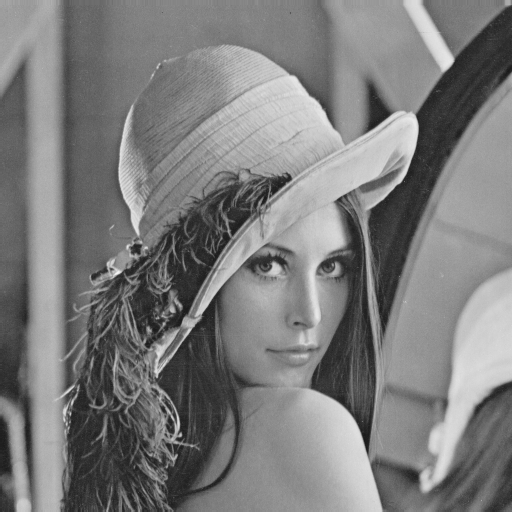
\includegraphics[height=2.5cm]{lenna.png} &

\includegraphics[height=2.5cm]{lenna0_10.png} &
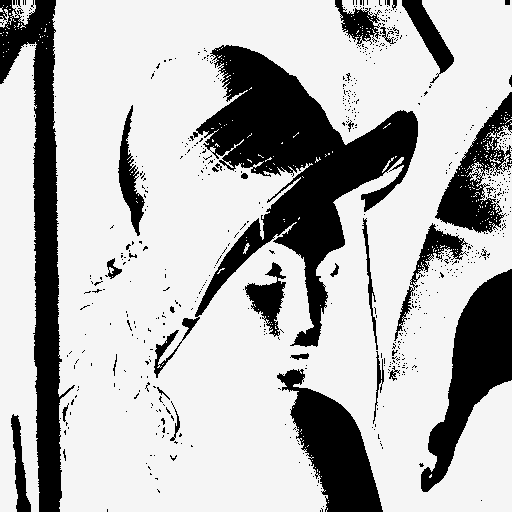
\includegraphics[height=2.5cm]{lenna0_25.png} &
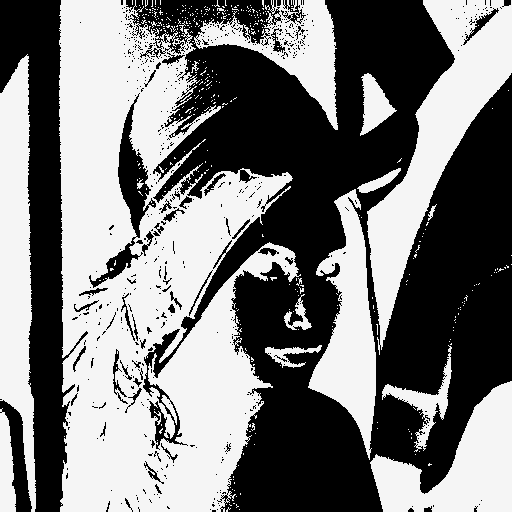
\includegraphics[height=2.5cm]{lenna0_50.png} &
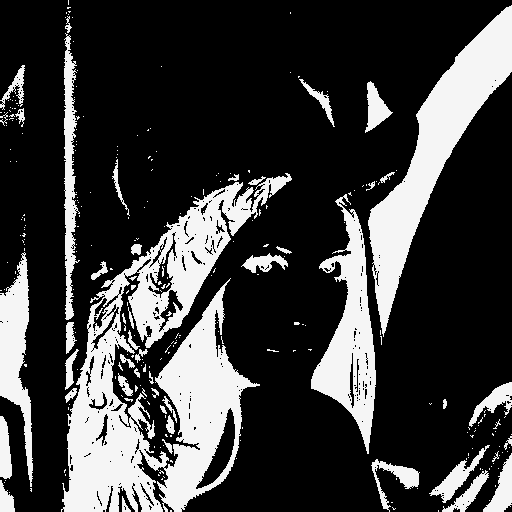
\includegraphics[height=2.5cm]{lenna0_75.png} &

\includegraphics[height=2.5cm]{lenna0_90.png} \\
Originale & 0.10 & 0.25 & 0.50 & 0.75 & 0.90 \\
\end{tabular}
\end{center}

Ovviamente potremmo utilizzare i modelli \textsf{Farm} e \textsf{Pipeline} per effettuare computazioni di una serie di immagini (ad esempio l'insieme di foto contenute in una cartella).




\section{Licence}
\small{
Tutto il codice sorgente scritto viene rilasciato sotto licenza Gnu GPL - General Public Licence versione 3, ognuno \`e libero di modificare e di distribuire il codice sorgente entro i termini di tale licenza.
Tale licenza pu\`o essere consultata all'indirizzo: http://www.gnu.org/copyleft/gpl.html

\begin{verbatim}
Copyright (C)  2013  Nicola Corti.
Permission is granted to copy, distribute and/or modify this document
under the terms of the GNU Free Documentation License, Version 1.3
or any later version published by the Free Software Foundation;
with no Invariant Sections, no Front-Cover Texts, and no Back-Cover Texts.
\end{verbatim}
Per qualsiasi problema \`e possibile contattare lo sviluppatore all'indirizzo e-mail \texttt{cortin [at] cli.di.unipi.it}.
}

\begin{landscape}
\appendix
\section{Grafici delle performance}
\label{appendix}
\subsection{Grafici delle performance di \textsf{Parallel}}


\begin{figure}[ht]
\centering
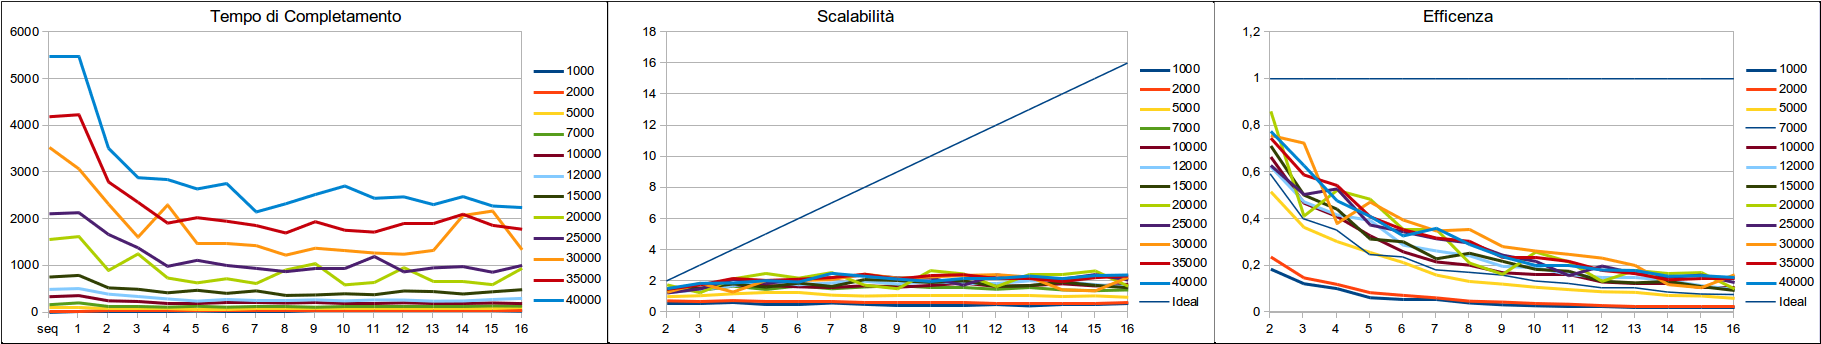
\includegraphics[height=3.9cm]{plot1.png}
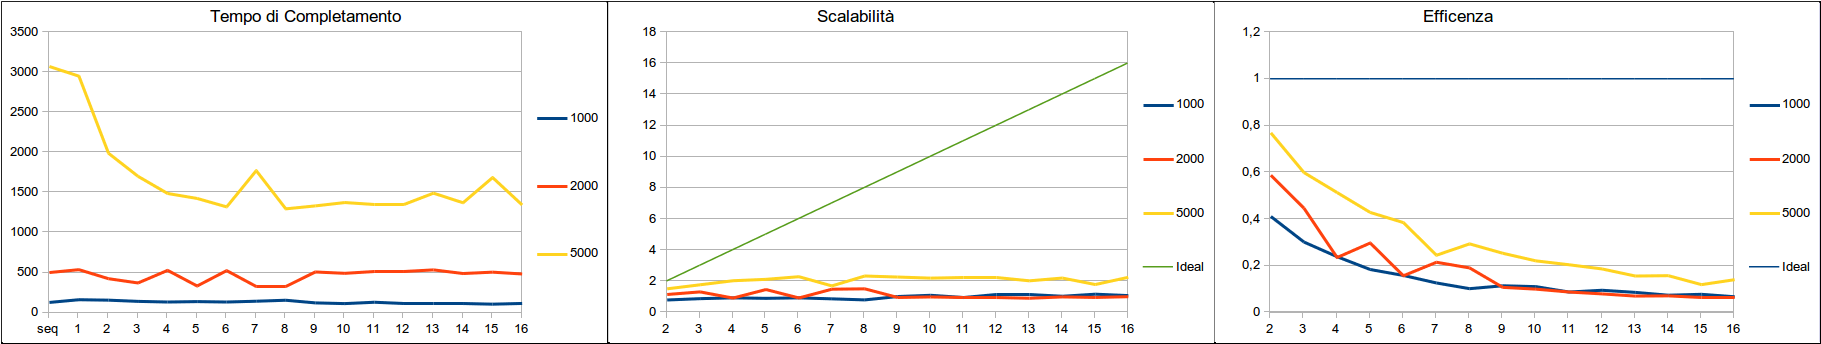
\includegraphics[height=3.9cm]{plot50.png}
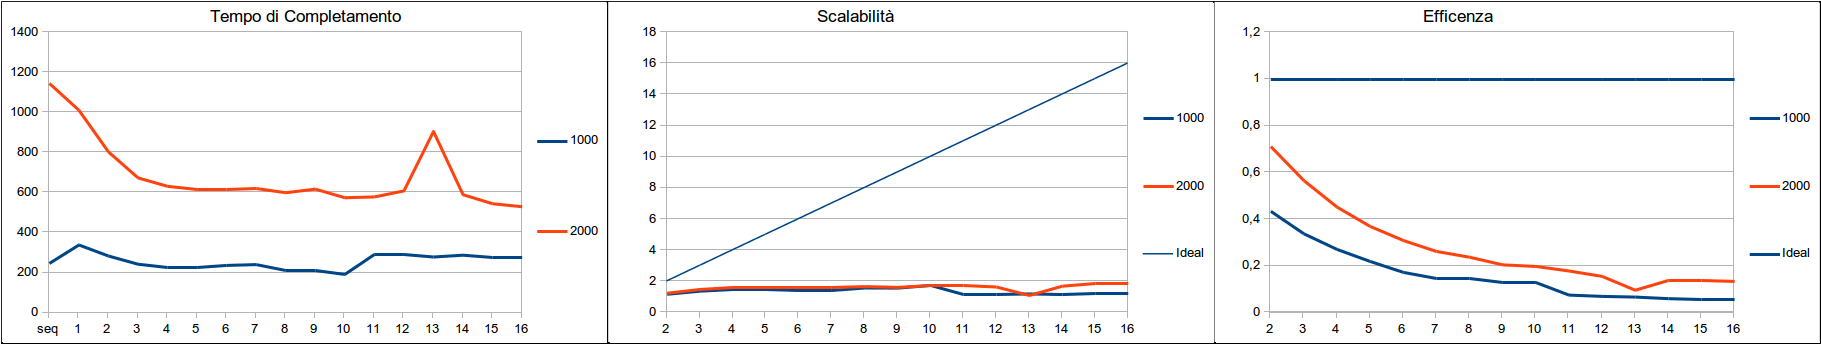
\includegraphics[height=3.9cm]{plot100.png}


\caption{\small{Grafici che mostrano tempo di completamento in millisecondi, scalabilit\`a e efficienza del modello \textsf{Parallel} (\textsf{Pipeline}). Sulla prima riga si possono vedere test effettuati su stream di una singola matrice con dimensioni che variano da $1000 \times 1000$ a $40.000 \times 40.000$. Sulla seconda e sulla terza riga si possono notare test effettuati su stream di lunghezza 50 e 100; si noti come le dimensioni delle matrici sono ridotte, in quanto la macchina su cui sono stati effettuati test aveva memoria limitata}}
\label{fig:par}
\end{figure}

Dai grafici si evince che, malgrado il tempo di completamento sia stato ridotto tramite l'esecuzione parallela, l'applicazione scala poco, riuscendo a raggiungere un valore prossimo a 2. Anche l'efficenza risulta molto bassa, anche se notiamo che aumenta, all'aumentare della dimensione della matrice; sarebbe stato interessante provare ed eseguire test con stream di lunghezza 50 e 100 e matrici di dimensione $40.000 \times 40.000$, ma la memoria a disposizione non era sufficiente.

Eventuali oscillazioni dei grafici (le ``punte'' che appaiono nel grafico del tempo di completamento) possono indicare calcoli che sono stati effettuati in momenti in cui la macchina non era completamente scarica da altri task, ma aveva in esecuzione altri processi che potevano tenere impegnati i processori e rallentare l'esecuzione. Per attenuare questo fenomeno avremo dovuto eseguire pi\`u calcoli in momenti differenti e calcolarne la media.


\subsection{Grafici delle performance di \textsf{ParallelFarm}}

\begin{figure}[ht]
\centering
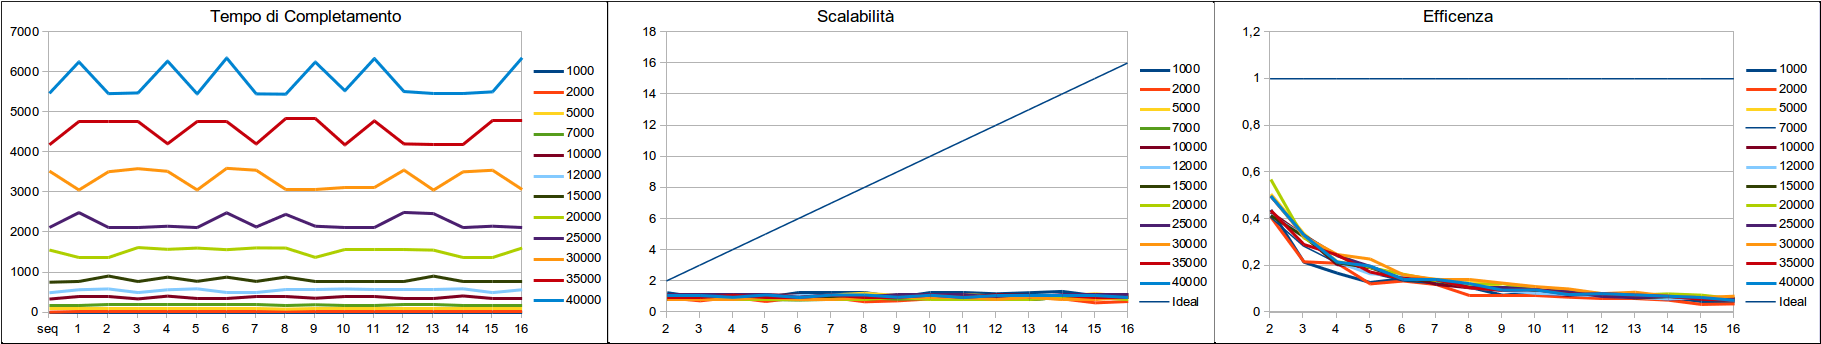
\includegraphics[height=4cm]{plot1farm.png}
\centering
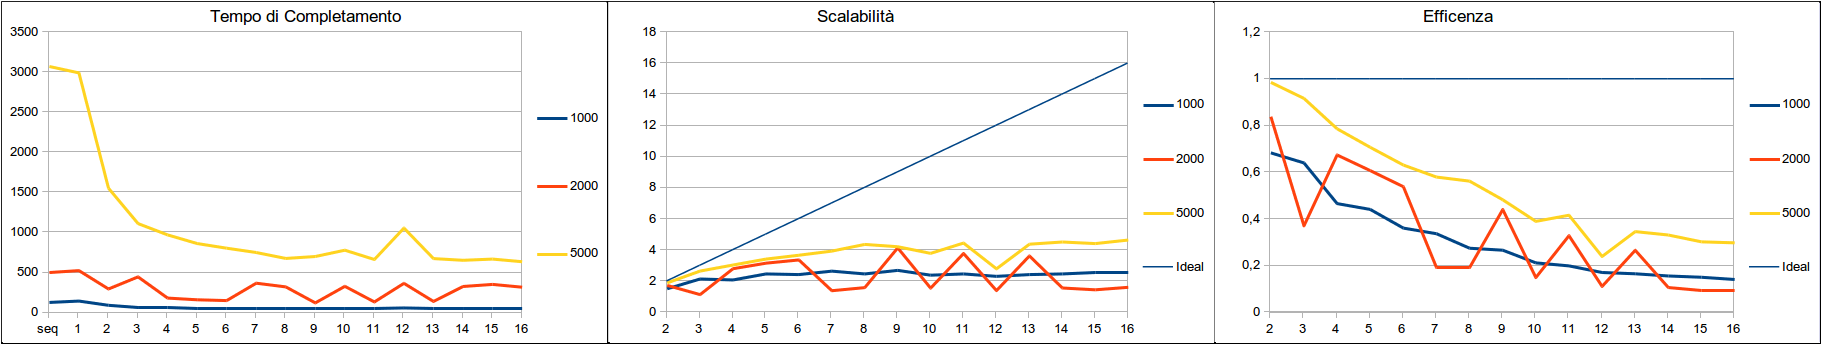
\includegraphics[height=4cm]{plot50farm.png}
\centering
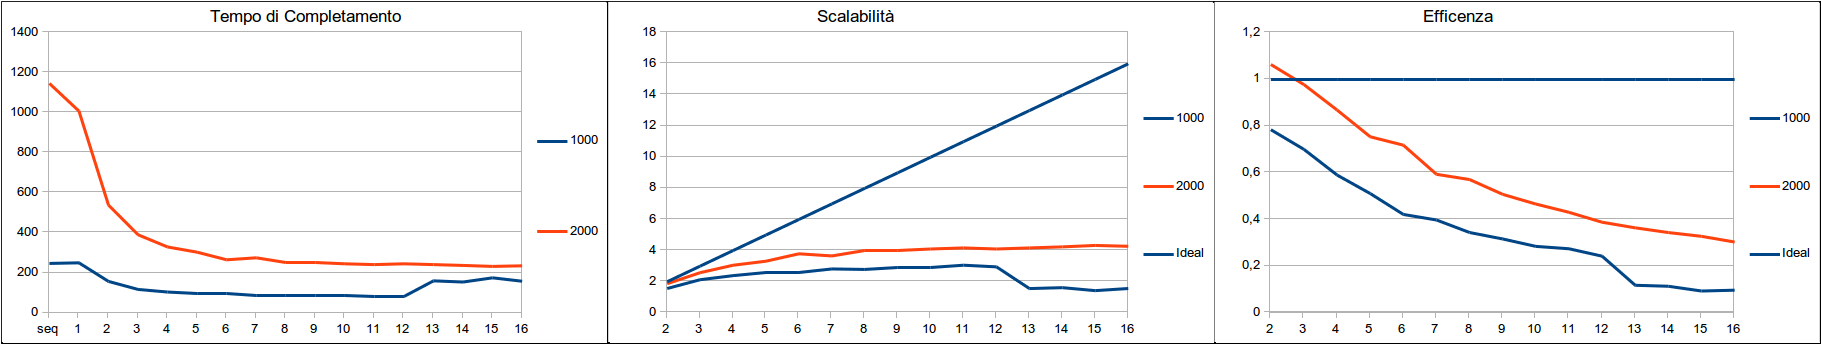
\includegraphics[height=4cm]{plot100farm.png}


\caption{\small{Grafici che mostrano tempo di completamento in millisecondi, scalabilit\`a e efficienza del modello \textsf{Farm}. Sulla prima riga si possono vedere test effettuati su stream di una singola matrice con dimensioni che variano da $1000 \times 1000$ a $40.000 \times 40.000$. Sulla seconda e sulla terza riga si possono notare test effettuati su stream di lunghezza 50 e 100; si noti come le dimensioni delle matrici sono ridotte, in quanto la macchina su cui sono stati effettuati test aveva memoria limitata.}}
\label{fig:farm}

\end{figure}

Dai grafici si evince che, come atteso, il modello \textsf{Farm} non \`e assolutamente adatto a calcoli con un singola matrice, il tempo di completamento risulta infatti costante per questi casi. Per quanto riguarda invece computazioni che coinvolgono stream di matrici si pu\`o notare che, malgrado il tempo di completamento sia stato ridotto tramite l'esecuzione parallela, l'applicazione scala poco, riuscendo a raggiungere un valore di scalabilit\`a prossimo a 2. Anche l'efficienza risulta molto bassa, anche se notiamo che aumenta, all'aumentare della dimensione della matrice. Sarebbe stato interessante provare ed eseguire test con stream di lunghezza 50 e 100 e matrici di dimensione $40.000 \times 40.000$, ma la memoria a disposizione non era sufficiente.

Per stream di lunghezza maggiore invece notiamo che si raggiungono risultati migliori del modello \textsf{Pipeline}, ad esempio per il caso con stream di lunghezza 100 e con matrici $2.000 \times 2.000$ si nota che si raggiunge un scalabilit\`a di 4 e che l'efficienza con grado di parallelismo 2 risulta essere superiore ad 1.

%Anche in questo caso sarebbe stato interessante fare prove su stream pi\`u lunghi e con matrici di maggiori dimensioni.


\subsection{Grafici delle performance di \textsf{ParallelQuad}}

\begin{figure}[ht]
\centering
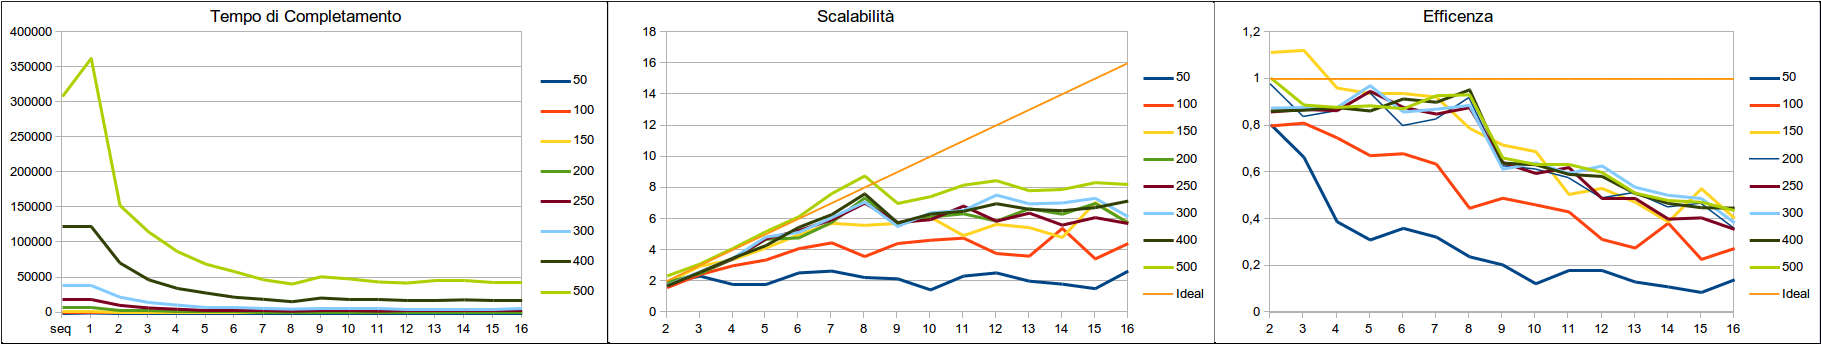
\includegraphics[height=3.9cm]{plot1quad.png}
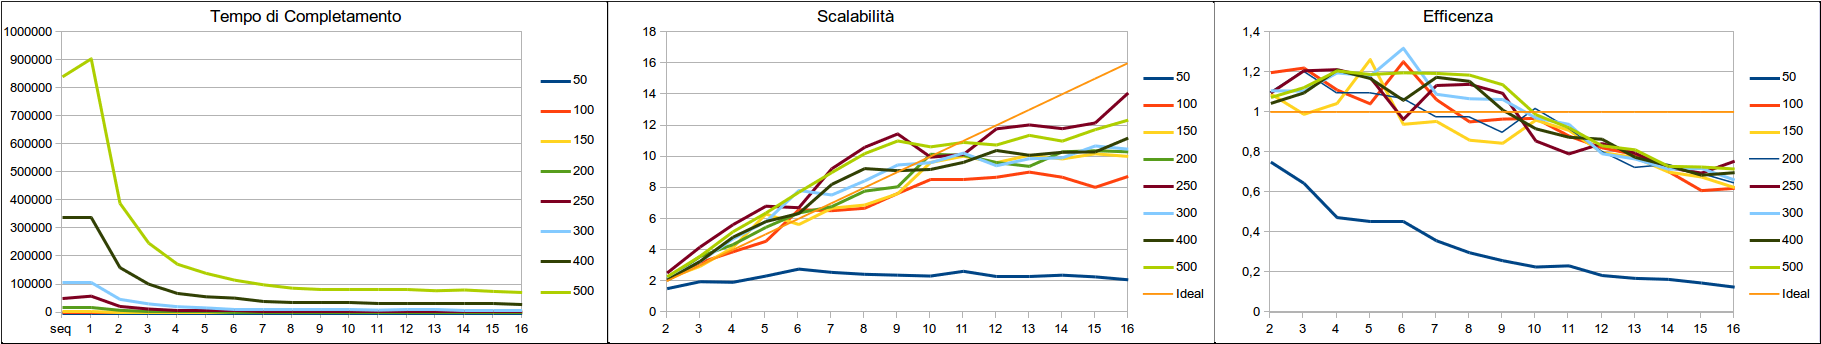
\includegraphics[height=3.9cm]{plot5quad.png}
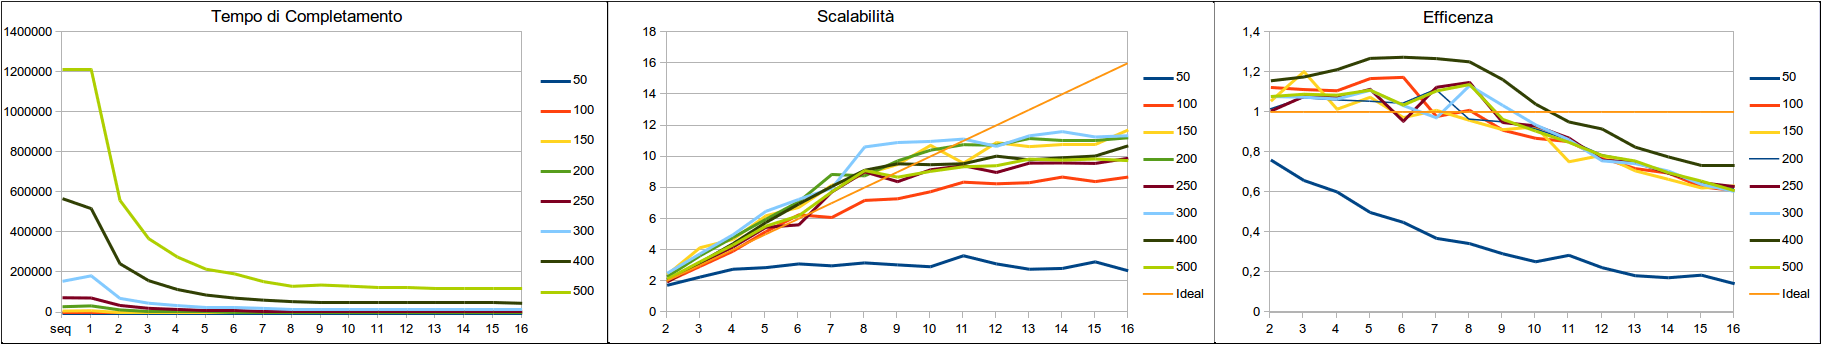
\includegraphics[height=3.9cm]{plot10quad.png}


\caption{\small{Grafici che mostrano tempo di completamento in millisecondi, scalabilit\`a e efficienza del modello \textsf{Map} utilizzando l'algoritmo quadratico. Sulla prima riga si possono vedere test effettuati su stream di una singola matrice con dimensioni che variano da $50 \times 50$ a $500 \times 500$. Sulla seconda e sulla terza riga si possono notare test effettuati su stream di lunghezza 5 e 10; le dimensioni sono notevolmente ridotte perch\'e il tempo impiegato per fare i test cresceva notevolmente.}}
\label{fig:quad}

\end{figure}

\normalsize{Come possiamo notare in questi grafici, il tempo di completamento in valore assoluto \`e molto pi\`u alto di quello ottenuto con i modelli \textsf{Pipeline} e \textsf{Farm} (si pensi che per calcolare uno stream di 10 matrici $500 \times 500$ sono necessari circa $1.200.000$ millisecondi, ovvero 20 minuti.

I risultati in termini di scalabilit\`a e di efficienza sono invece pi\`u che ottimi, si riesce ad ottenere un risultato \emph{super-lineare} infatti si nota che la scalabilit\`a ottenuta \`e maggiore di quella indicata dalla linea ideale.

Ne consegue che si ottengono efficienze superiori ad 1, come dimostrato dai grafici dell'efficienza.

Si noti come l'efficienza rimanga pressoch\'e stabile fino ad un grado di parallelismo pari ad 8 e poi tenda a decadere (un evento simile si pu\`o riscontrare anche nel grafico della scalabilit\`a); ci\`o pu\`o essere dovuto al fatto che la macchina aveva 8 core con 2 contesti, per cui da grado di parallelismo 9 in su inizia ad eseguire thread su due contesti di uno stesso core, andando a perdere in performance}


\end{landscape}

\end{document}
